	\documentclass[12pt,a4paper,openright]{report}
	\usepackage{bm}
	\usepackage{geometry}
	\usepackage[T1]{fontenc}
	\usepackage{amsfonts}
	\usepackage{relsize}
	\usepackage[Lenny]{fncychap}
	\makeatletter
	\def\mathbi#1{\textbf{\em #1}}
	\def\@makeschapterhead#1{%
		\vspace*{0\p@}%
		{\parindent\z@\raggedright\normalfont\interlinepenalty\@M
			\DOTIS{#1}%
			\vskip-30\p@ 
			\kern-.4\p@
			\vskip0\p@}%
	}
	\makeatother
	\usepackage{verbatim}
	\usepackage{algorithm}
	\usepackage{algpseudocode}
	\usepackage{listings}
	\usepackage{etoolbox}
	\makeatletter
	\patchcmd{\l@chapter}{\bfseries}{}{}{}
	\makeatother
	\usepackage{empheq}
	\usepackage{longtable}
	\geometry{
		a4paper,
		left = 25.5mm,
		top = 0mm,
		bottom = 25.5mm,
	}
	\usepackage{amsmath, amsthm, amssymb}
	%\usepackage{nomencl}
	\usepackage{epstopdf}
	\usepackage{caption}
	\usepackage{float}
	\usepackage{latexsym}
	\usepackage{array}
	\usepackage{acronym}
	\usepackage{setspace}
	\usepackage{fancyhdr}
	\usepackage{xcolor}
	\usepackage{multicol}
	\usepackage{lipsum}
	\usepackage{verbatim}
	\usepackage{layaureo}
	\usepackage{chngpage}
	\usepackage{amsfonts}
	\usepackage{makeidx}
	\makeindex
	\usepackage{enumerate}
	\usepackage{calligra}
	\usepackage[font={footnotesize}]{caption}
	\usepackage[scr=boondoxo,
	scrscaled=1.15,]{mathalfa}
	\usepackage{multirow}
	\usepackage{cite}
	\usepackage{graphicx}
	\usepackage{url}
	\usepackage[bookmarks, colorlinks=false, pdfborder={0 0 0}, pdftitle={<pdf title here>}, pdfauthor={<author's name here>}, pdfsubject={<subject here>}, pdfkeywords={<keywords here>}]{hyperref} 
	
	\begin{document}
		\begin{titlepage}
			
			\begin{center}
				\Huge{\textbf{MAKERERE}}
\includegraphics[width=0.2\textwidth]{logo.png}\Huge{\textbf{UNIVERSITY}}\\[0.5in]
				\Large
				COLLEGE OF ENGINEERING, DESIGN, ART \& TECHNOLOGY\\[0.3in]
				SCHOOL OF ENGINEERING\\[0.3in]
				\large{DEPARTMENT OF ELECTRICAL \& COMPUTER ENGINEERING} \\[.5in]
				
				% Title
				\Large \textbf {Assignment 1}\\[.3in]
				\Large \textbf {Transmission Lines}\\[.5in]
				
				
				
				% Submitted by
				\normalsize Submitted by \\[0.2in]
				\textbf{Kakooza Abraham Jerry}\\
				16/U/327\\
				216000136\\
				
				\vspace{.5in}
				\Large \textbf {Group Members}\\[.1in]
				
				\begin{table}[H]
					\begin{center}
						%\caption{Group Members}\label{table1}
						\begin{tabular}{|l|l|}
							\hline
							Name & Reg. No.\\ \hline
							Kakooza Abraham Jerry & 16/U/327 \\ \hline
							Mbarebaki Adonai & 16/U/ \\ \hline
							Peter Claver & 16/U/ \\ \hline
							Akhol Peter & 16/U/ \\ \hline
						\end{tabular}
					\end{center}
				\end{table}
				
				
				\vfill
				\normalsize
				$19^{th}$ October, 2020
				
				% Bottom of the page
				
				
			\end{center}
			
		\end{titlepage}
	
	\begin{enumerate}
		\noindent \section*{Solution to Question 1}
		\item Given the figure below
		\begin{figure}[H]
			\centering
			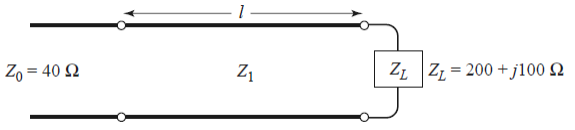
\includegraphics[width=11.3cm,height=5cm]{figure1.png}
			%\caption{
				%SOP against the overall average transmit power with $A_{J}=3$, $N_{A}=3$, $M_{BE}=5$, $\phi=0.9$, $N_{E}=10$ and $N_{B}=2$.	
			%}
			\label{F1}
		\end{figure}
		\begin{align*}
		Z_{\mathbf{in}}=Z_{\mathbf{0}}=40\Omega
		\end{align*}
		
		\begin{align*}
		Z_{\mathbf{in}}=Z_{\mathbf{1}}\biggl(\frac{Z_L+jZ_1{\tan}{\beta}l}{Z_1+jZ_L{\tan}{\beta}l}\biggr),
		\end{align*}
		let $t={\tan}{\beta}l$ such that
		
		\begin{align*}
		Z_{\mathbf{in}}=Z_{\mathbf{1}}\biggl(\frac{(200+i100)+jZ_1t}{Z_1+j(200+i100)t}\biggr),
		\end{align*}
		
		\begin{align*}
		(40Z_{1}-4000t)+j8000t=200Z_{1}+j(100+Z_{1}t)Z_{1}
		\end{align*}
		
		Equating real and imaginary factors
		\\
		Re:
		\begin{align*}
		40Z_{1}-4000t&=200Z_{1}\\\notag\\160Z_{1}&=-4000t\\\notag\\Z_{1}&=-25t
		\end{align*}
		\\
		Im:
		\begin{align*}
		5000t&=Z_{1}(100+Z_{1}t)\\\notag\\8000t&=-25t(100-25t)\\\notag\\\8000t&=-2500t+625t^{3}\\\notag\\t(625t^{2}-10500)&=0
		\end{align*}
		\\
		Either $t=0$
		\\
		Or 
		\begin{align*}
		(625t^{2}-10500)&=0\\\notag\\t&=\pm\sqrt{16.8}\\\notag\\t&=\pm4.1
		\end{align*}
		
		Therefore $t=-4.1$, so that $Z_{1}=102.5\Omega$
		
		From $t=\tan\beta{l}$
		
		\begin{align*}
		\beta{l}&=\arctan{t}=\arctan{-4.1}=-76.3^{\circ}\Leftrightarrow{104^{\circ}}
		\end{align*}
		
		$\therefore$
		
		\begin{align*}
		\frac{2\pi{l}}{\lambda}&=104\\\notag\\l&=0.289\lambda
		\end{align*}
		\noindent \section*{Solution to Question 2}
		\item Given the figure below
		
		\begin{figure}[H]
			\centering
			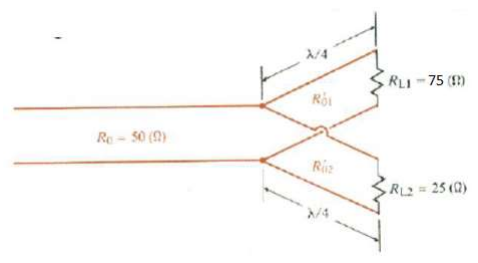
\includegraphics[width=11.3cm,height=5cm]{figure2.png}
			%\caption{
			%SOP against the overall average transmit power with $A_{J}=3$, $N_{A}=3$, $M_{BE}=5$, $\phi=0.9$, $N_{E}=10$ and $N_{B}=2$.	
			%}
			\label{F1}
		\end{figure}
	
		\begin{enumerate}
			\item The input impedance of the two branch looking at the junction from the $50\Omega$ line must be equal to $100\Omega$ such that when they are in parallel the resultant impedance is $50\Omega$
			
			\begin{figure}[H]
				\centering
				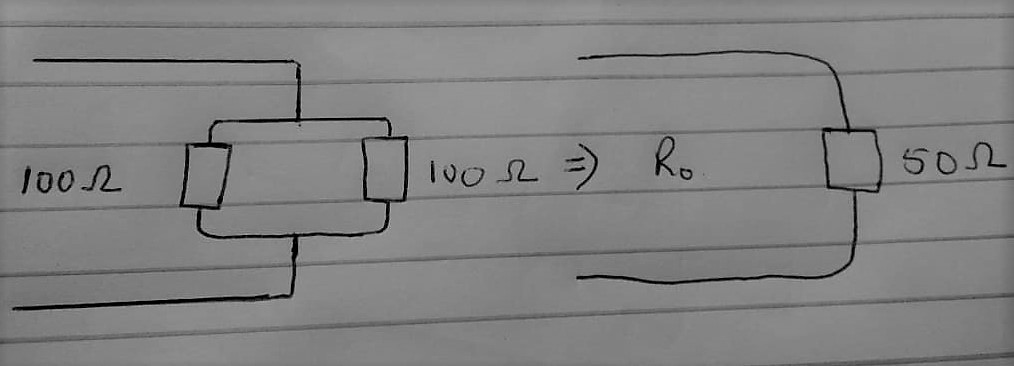
\includegraphics[width=11.3cm,height=5cm]{fig4.jpeg}
				%\caption{
				%SOP against the overall average transmit power with $A_{J}=3$, $N_{A}=3$, $M_{BE}=5$, $\phi=0.9$, $N_{E}=10$ and $N_{B}=2$.	
				%}
				\label{F1}
			\end{figure}
			
			\begin{align*}
			Z_\mathbf{in_1}=R_\mathbf{in_1}=100\Omega
			\end{align*}
			\\
			The characteristics impedance
			
			\begin{align*}
			R_{o_1}=\sqrt{R_\mathbf{in_1}R_\mathbf{L_1}}=\sqrt{100\times75}=86.6\Omega
			\end{align*}
			\\
			Similarly
			
			\begin{align*}
			R_{o_2}=\sqrt{R_\mathbf{in_2}R_\mathbf{L_2}}=\sqrt{100\times25}=50\Omega
			\end{align*}
			\\
			Physical length, $l_{P}=0.5c$
			\\
			\\
			From
			
			\begin{align*}
			\frac{1}{\sqrt{\mu_{o} \varepsilon}}&=\medspace 0.5c\\\linebreak\\\notag\frac{1}{\sqrt{\mu_{o} \varepsilon_{o}\varepsilon_{r}}}&=\medspace 0.5c\\\linebreak\\\notag\varepsilon_{r}&=\medspace\frac{4}{\mu\varepsilon_{r}c^2}\\&\notag=\frac{4}{8.85\times10^{-12}\times1.26\times10^{-6}\times(3\times10^{8})^2}\\\linebreak\\\notag\varepsilon_{r}&=\medspace 4
			\end{align*}
			\\
			Wavelength along the transformers
			
			\begin{align*}
			\lambda&=\frac{0.5c}{f}\\&\notag=\frac{0.5\times3\times10^8}{100\times10^6}\\&\notag=\medspace1.5m
			\end{align*}
			\\
			Physical length of the transformers
			\begin{align*}
			\frac{\lambda}{4}&=\frac{1.5}{4}=\medspace 0.375m
			\end{align*}
			
			\item When matched, $SWR=1$, on the main transmission line
			\begin{align*}
			\Gamma_{L_1}&=\frac{R_\mathbf{L_1}-R_\mathbf{o_1}}{R_\mathbf{L_1}+R_\mathbf{o_1}}\\\medskip\\&\notag=\frac{75-86.6}{75+86.6}=-0.072
			\end{align*}
			
			\begin{align*}
			SWR_{1}&=\frac{1+\vert\Gamma_{L_1}\vert}{1-\vert\Gamma_{L_1}\vert}\\\medskip\\&\notag=\frac{1+0.072}{1-0.072}=1.16
			\end{align*}
			\\
			Similarly
			\begin{align*}
			\Gamma_{L_2}&=\frac{R_\mathbf{L_2}-R_\mathbf{o_1}}{R_\mathbf{L_2}+R_\mathbf{o_1}}\\\medskip\\&\notag=\frac{25-50}{25+50}=-0.33
			\end{align*}
			
			\begin{align*}
			SWR_{2}&=\frac{1+\vert\Gamma_{L_2}\vert}{1-\vert\Gamma_{L_2}\vert}\\\medskip\\&\notag=\frac{1+0.33}{1-0.33}=1.99
			\end{align*}
		\end{enumerate}
	\end{enumerate}

    \end{document}